\section{Adaptive Profiling: Promise and Challenge}

Our first insight is that the performance of video analytics systems
can be remarkably improved by {\em adaptive profiling}, whereby we 
continously profiling the resource-accuracy tradeoffs and dynamically
picking the optimal configuration.
This section first describes a high-level overview of adaptive 
profiling, then empirically shows its potential improvement over 
baseline solutions, and finally discuss the challenge towards 
realizing such potential improvement.

\subsection{Overview of \name}

Figure~\ref{fig:overview} shows the high-level design of {\em \name},
a video analytics system that is capable of adaptive profiling, and 
its contrast with prior solutions.
What is new in adaptive profiling are two-fold. 
First, during the process of a query, we may choose to switch to a
different configuration that strikes a better balance than the 
previous one between accuracy and resource consumption given the 
available resource. 
Second, at the core of \name is {\em \name control algorithm}, which 
decides what which configuration is used in each query at any moment.
Note that this design is not specific to any specific underlying \nn 
model.

The key feature that distinguishes \name from prior systems is that
\name profiles the resource-accuracy tradeoffs of various 
configurations in an online fashion, whereby prior solutions profile
the resource-accuracy tradeoffs once for each query in an offline 
fashion.
This allows \name to dynamically identify the optimal configuration
when the configurations have dynamic resource-accuracy tradeoffs.
At the same time, it also introduces the additional cost of 
continuous profiling, which will be discussed in \Section\ref{?}

\subsection{Potential improvement}
We first empirically show the potential improvement by adaptive 
profiling.
That is, compared to using the same configuration over time, how much
we can improve performance, if we know the optimal configurations for
each query at any moment and there is no cost associate to 
identifying the optimal configuration.
Since prior work 

In Figure~\ref{fig:potential}, we applied Yolo~v2 object detector on
120 traffic camera videos, each of 2.5 minutes. 
We considered three configurations: sampling rate, brightness,
and Yolo input resolution.
\jc{show the results here}

%\begin{figure}[h!]
%\centering
%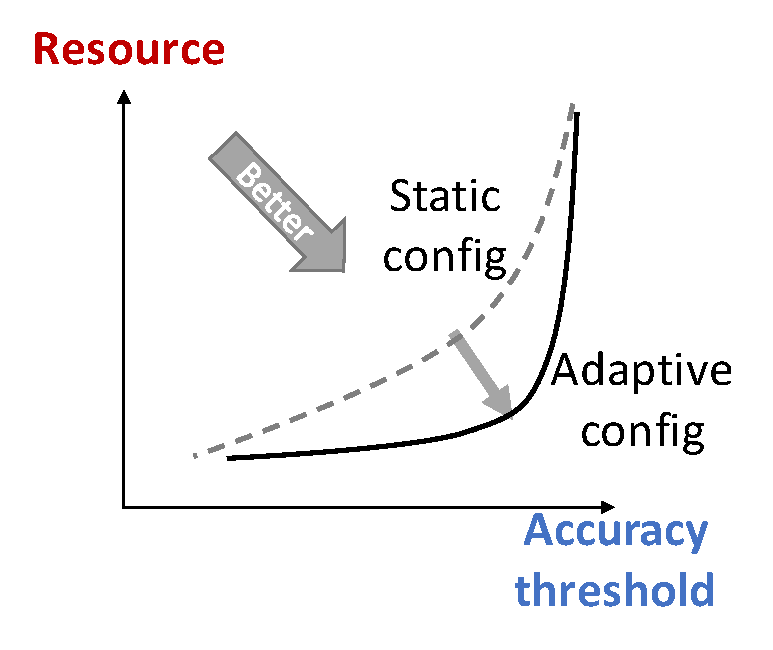
\includegraphics[width=0.35\textwidth]{figures/OraclePotential.pdf}
%\vspace{-0.2cm}
%\tightcaption{Potential improvement of adaptive profiling.}
%\label{fig:AdaptiveConfig}
%\end{figure}



\begin{figure}[t!]
\captionsetup[subfigure]{justification=centering,farskip=-1pt,captionskip=5pt}
\centering
\hspace{-0.5cm}
\subfloat[Camera \#1, Hour \#1, Accuracy threshold = 0.9$\cdot$MaxAccuracyOfEachFrame]
{
        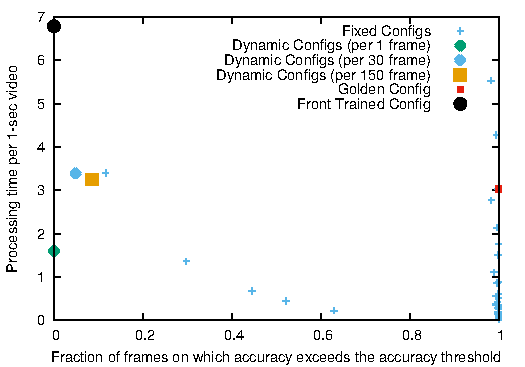
\includegraphics[width=0.45\textwidth]{PotentialFigures/OverallTradeoffBellevue_116th_NE12th__2017-04-07_13_Tolerance_1.pdf}
        \label{fig:eval-overall-quality-jointime}
}
\hspace{-0.4cm}
\subfloat[Camera \#1, Hour \#1, Accuracy threshold = 0.8$\cdot$MaxAccuracyOfEachFrame]
{
        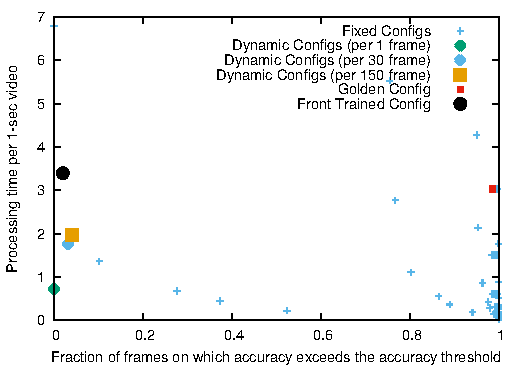
\includegraphics[width=0.45\textwidth]{PotentialFigures/OverallTradeoffBellevue_116th_NE12th__2017-04-07_13_Tolerance_2.pdf}
        \label{fig:eval-overall-quality-jointime}
}
\hspace{-0.4cm}
\subfloat[Camera \#2, Hour \#2, Accuracy threshold = 0.9$\cdot$MaxAccuracyOfEachFrame]
{
        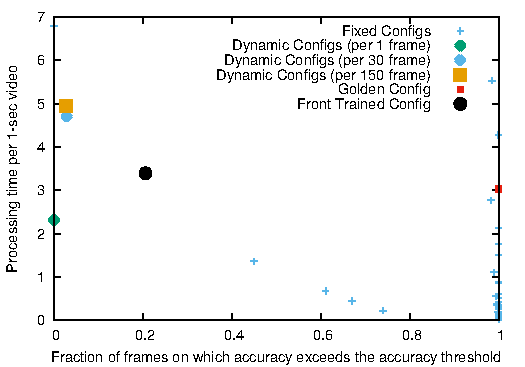
\includegraphics[width=0.45\textwidth]{PotentialFigures/OverallTradeoffBellevue_116th_NE12th__2017-04-07_15_Tolerance_1.pdf}
        \label{fig:eval-overall-quality-jointime}
}
\hspace{-0.4cm}
\subfloat[Camera \#3, Hour \#3, Accuracy threshold = 0.6$\cdot$MaxAccuracyOfEachFrame]
{
        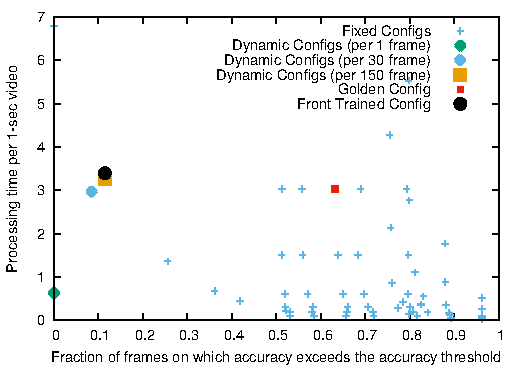
\includegraphics[width=0.45\textwidth]{PotentialFigures/OverallTradeoffBellevue_116th_NE12th__2017-04-08_01_Tolerance_4.pdf}
        \label{fig:eval-overall-quality-jointime}
}
\hspace{-0.4cm}
\vspace{-0.2cm}
\tightcaption{Dynamic selection of configurations (at various timescales) vs. static configurations vs. golden configuration vs. ``front-training'' approach.}
%\vspace{-0.2cm}
\label{fig:eval-overall-quality}
\end{figure}

\subsection{Challenge of exploration cost}
While adaptive profiling is very promising, to realize its full 
potential \name must identify the optimal configuration with minimal
{\em exploration cost}, which breaks down to two parts.
First, \name must monitor the amount of available resource, so that
given the resource-accuracy tradeoffs of different configuration, 
it will be able to identify the best configuration under the resource
constraint. 
Second, \name needs to reprofile the resource-accuracy tradeoffs of 
configurations, so that as they drift over time, we can identify the
optimal configuration over time.

Here, we use one-second worth of video to microbenchmark the second 
cost of reprofiling the resource-accuracy tradeoffs, and we consider
three configurations with the following values.
\jc{show the results here}

In short, adaptive profiling could remarkably improvement the 
performance of video analytics systems by enabling dynamic picking
of optimal configurations, but realizing its potential introduces
a potentially prohibitive cost of exploration, which we seek to 
trim in the next section.
